\documentclass{article}
\usepackage[utf8]{inputenc}
\usepackage{graphicx}
\usepackage{mathtools} 
\usepackage{textcomp}
\usepackage{titling}
\usepackage{subfig}
\usepackage{amsmath}
\usepackage[parfill]{parskip}
\usepackage{xcolor}
\definecolor{LightGray}{gray}{0.9}
\usepackage{titlesec}
\setcounter{secnumdepth}{4}
\usepackage[a4paper,left=1cm,right=1cm,top=1cm,bottom=1.5cm,]{geometry}

\title{\vspace{-2cm} EE4218 L3 - State Machine Optimization}
\date{\vspace{-5ex}}

\begin{document}
\maketitle

\section{Modelling Synchronous Circuits}
There are two main ways to model synchronous circuits; State-based models or Structural models.
\begin{itemize}
    \item State-based model $\xrightarrow{\text{State Encoding}}$ Structural model
    \item Structural model $\xrightarrow{\text{State Extraction}}$ State-based model
\end{itemize}


\subsection{State-based Model (ie. Behavioral Modelling)}
Typically modelled using state-transition graphs.


\begin{itemize}
    \item Model circuits as \textbf{FINITE-STATE MACHINES}
    \item Represent behavior via state-table/diagrams
    \item Explicit notion of state, implicit notion of area/timing
    \item State-based optimizations are...
        \begin{enumerate}
            \item State Minimization (Merging similar states)
                \begin{itemize}
                    \item If two states are identical, there is no need for us to implement both of them
                \end{itemize}
            \item State encoding (Assigning binary patterns to the symbolic states)
                \begin{itemize}
                    \item Represents the \textit{symbolic} state function as a Boolean function, 
                          which can be implemented with \textit{actual} hardware
                \end{itemize}
        \end{enumerate}
\end{itemize}

\begin{figure}[htp]
    \centering
    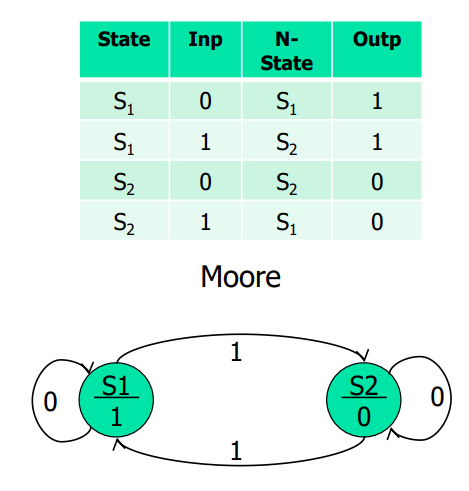
\includegraphics[width=5cm, scale=1]{S1/stateBasedModelling.PNG}
    \caption{Example of State-based modelling of a Moore machine}
\end{figure}

\subsection{Structural Modelling}
Represent the circuit using \textit{synchronous logic network}.

\begin{itemize}
    \item Explicit notion of area/timing, implicit notion of state
    \item Structural-based optimizations are...
        \begin{enumerate}
            \item Retiming
            \item Synchronous logic transformations (Not covered)
        \end{enumerate}
\end{itemize}

\begin{figure}[htp]
    \centering
    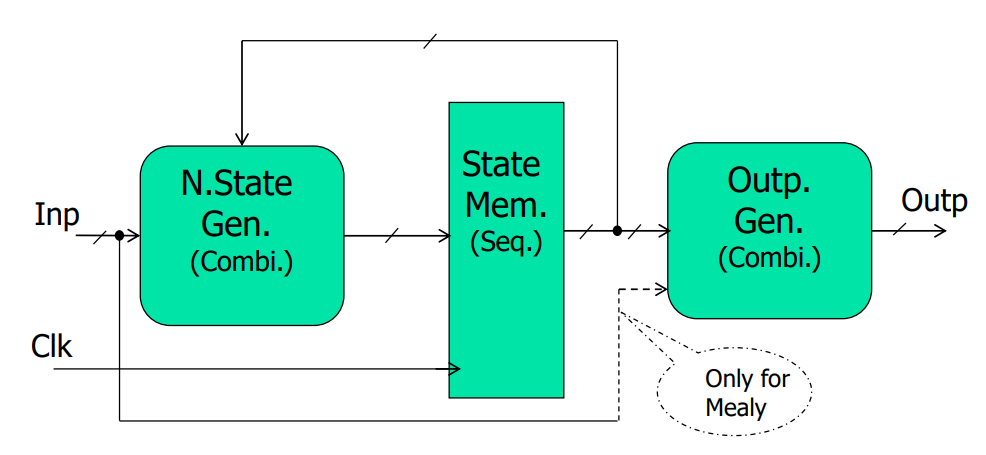
\includegraphics[width=8cm, scale=1]{S1/structuralBasedModelling.PNG}
    \caption{Generic structural model}
\end{figure}

Note that we will see how to transform the structural model of Fig2 into a synchronous logic network later.

\newpage

\section{State Machine Optimization}
Assumptions
\begin{itemize}
    \item Single-phase clocking
    \item No combinational feedback loops in the circuit (We operate at a higher abstraction level)
        \begin{itemize}
            \item eg. In Fig3 below, a latch involves combinational feedback paths (to implement Memory)
            \item However, we view the latch as a black-box unit
        \end{itemize}
        \begin{figure}[htp]
            \centering
            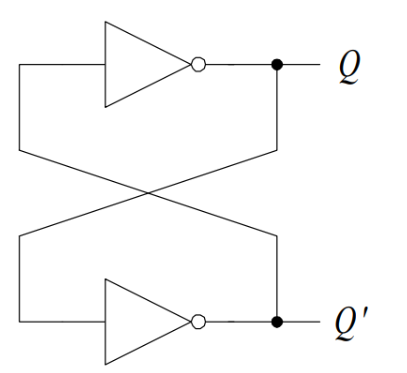
\includegraphics[width=2cm, scale=1]{S2/bistableElement.PNG}
            \caption{Bistable element used in latches}
        \end{figure}
\end{itemize}

\subsection{Optimization flow}
\begin{enumerate}
    \item FSM specification (ie. Algorithmic procedure to solve a problem)
    \item State Minimization
    \item State Encoding (Moving from State-based to Structural-based)
    \item \textbf{COMBINATIONAL} logic optimization
        \begin{itemize}
            \item Combinational \underline{next-state} logic optimization
            \item Combinational \underline{output} logic optimization
        \end{itemize}
    \item State Extraction (Moving back from Structural-based to State-based)
        \begin{itemize}
            \item Recovers state information from structural model, to verify the structural model
        \end{itemize}
    \item Retiming and synchronous transformations
        \begin{itemize}
            \item For the synchronous portion of the State Machine
        \end{itemize}
\end{enumerate}

\subsection{State Encoding}
Lets cover State Encoding first, i.e Converting from State-based model to Structural-based model.

\vspace{0.5cm}
As seen in Fig4, structural modelling is not unique. Which circuit is better depends on the PPA requirements.
\begin{figure}[htp]%
    \centering
    \subfloat[\centering State Encoding 1]{{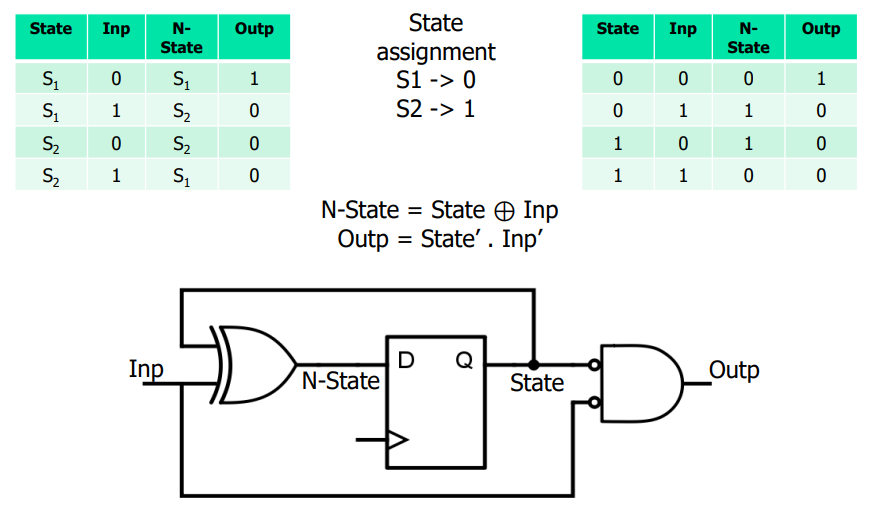
\includegraphics[width=9cm]{S2/stateEncoding1.PNG}}}% 
    \qquad
    \subfloat[\centering State Encoding 2]{{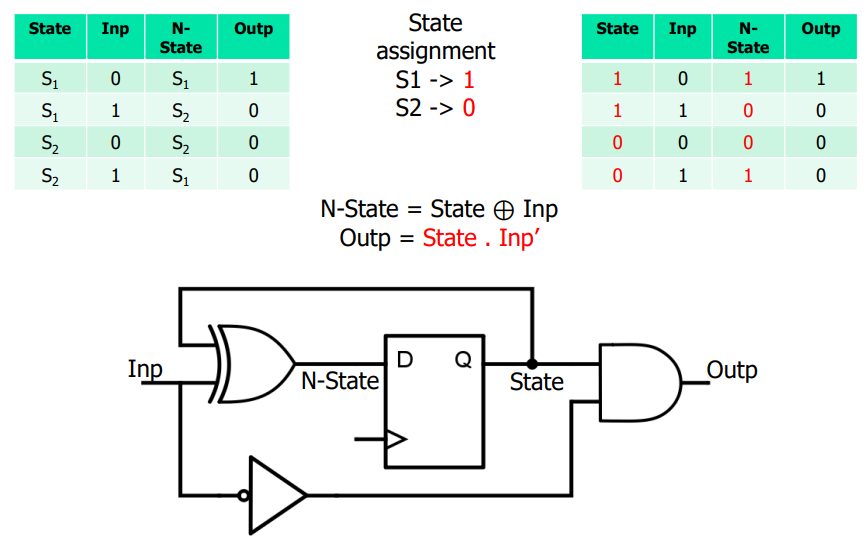
\includegraphics[width=9cm]{S2/stateEncoding2.PNG}}}% 
    \caption{Non-uniqueness of Structural models}%
\end{figure}

\newpage
\subsection{State Minimization}
Objective is to reduce the number of states (and hence the hardware area)

Note that the complexity of State Minimization depends on the \textbf{degree} of FSM specification
\begin{itemize}
    \item Completely-specified FSM's (CS-FSM)
        \begin{itemize}
            \item No don't-care condition(s)
            \item There are polynomial time solutions to do state minimization
        \end{itemize}
    \item Incompletely-specified FSM (IS-FSM)
        \begin{itemize}
            \item $\exists$ don't-care condition(s); Therefore there are unspecified transitions and/or outputs
            \item Problem is intractable (NP). We have to brute-force iterate through all possible combinations of the X's, to see which scenario is best
        \end{itemize}
\end{itemize}

\subsubsection{What's the deal with don't-cares?}
They complicate analysis of the system.

Fig5 is an example of how don't cares increase complexity (in the context of logic simplification, not state minimization).

\begin{figure}[htp]
    \centering
    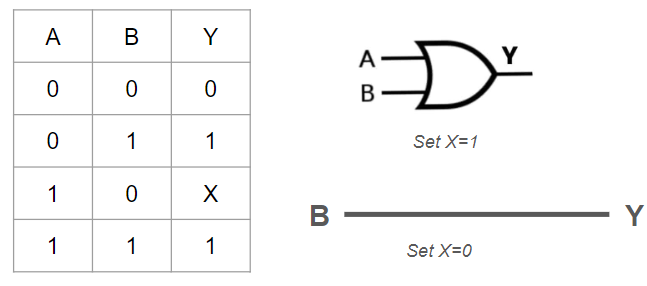
\includegraphics[width=10cm, scale=1]{S2/dontCares.PNG}
    \caption{Hardware implementation is simplified, if we set X=0}
\end{figure}

\begin{itemize}
    \item 
        Don't-cares in the output means that the output was not specified (ie. Output can randomly be 0 or 1, it does not affect system functionality).
        It does not mean that the output doesn't change. 

        Why?
        Because recall that if output doesn't change when input changes, it implies that the system has memory.
        Since truth tables are implementing combinational logic, we cannot have any form of memory.
    \item 
        More complicated scenarios can be tackled with K-maps.

    \item 
        Recognize that the inclusion of X's means that we have to try out every possible combination of X's
        to find out which scenario gives us the 'best' circuit. There is no polynomial time method.
\end{itemize}

\vspace{0.1cm}
Lets move back to the context of state minimization now.

For an IS-FSM, each X denotes two (X=0, X=1) possible CS-FSMs.
We must then state-minimize each CS-FSM using the polynomial time methods, before comparing
across all permutations of the CS-FSMs to find the solution for state-minimizing the original IS-FSM.

\subsubsection{State Minimization - Completely specified FSMs}
Note: The resulting "minimized" FSM is \textbf{unique}.

\paragraph{Concept of \textit{equivalent} states}
\begin{itemize}
    \item Assume we have two states $S_{1}$ and $S_{2}$. $S_{1}$ and $S_{2}$ defined as \textit{equivalent} iff for some input sequence\dots
        \begin{itemize}
            \item Their (combinational) outputs are identical, and
            \item Their (combinational) next-states are \textit{equivalent} (note the recursiveness) as well
        \end{itemize}
    \item Note that equivalence is \textit{transitive}
        \begin{itemize}
            \item $S_{1}$ is equivalent to $S_{2}$ $\wedge$ $S_{2}$ is equivalent to $S_{3}$ $\longrightarrow$  $S_{1}$ is equivalent to $S_{3}$
        \end{itemize}
\end{itemize}

\newpage
\paragraph{Algorithm for State Minimization of CS-FSMs}
\begin{enumerate}
    \item $\Pi_{0}$ : Initial partition.
        \begin{itemize}
            \item Assume that all states $ \left\{ S_{1}, S_{2}, \dots, S_{k} \right\} $ are equivalent
            \item This means that our FSM is a \textit{combinational-only} machine (combinational machines have no concept of states; ie. All next-states are equivalent)
                  that produces the same output for all inputs
            \item This is too optimistic an assumption, so we will refine it accordingly below...
        \end{itemize}
    \item $\Pi_{1}$ : Partition based on Output.
        \begin{itemize}
            \item We consider $ \left\{ S_{i},S_{j} \right\} $ to be equivalent iff for some input, their outputs are identical
            \item Partition $ \left\{ S_{1}, S_{2}, \dots, S_{k} \right\} $ accordingly
        \end{itemize}
    \item $\Pi_{k}, k \ge 2$ : Iterative partitioning. 
        \begin{itemize}
            \item $ \left\{ S_{i},S_{j} \right\} $ were equivalent in $\Pi_{k-1}$ $\wedge$ 
                  $ \left\{ S_{m},S_{n} \right\} $ (next states of $ \left\{ S_{i},S_{j} \right\} $) were equivalent in $\Pi_{k-1}$ for some input
                  $\longrightarrow$ $ \left\{ S_{i},S_{j} \right\} $ are considered "truly" equivalent now.
            \item Keep repeating until we reach convergence (Suppose $S_{i}$ and $S_{j}$ which were previously in the same block for $\Pi_{k-2}$ were changed to be in different blocks for $\Pi_{k-1}$.
                    Then during $\Pi_{k}$, we just need to re-check equivalence for any states $S_{k}$ that had $S_{i}$ or $S_{j}$ as their next-states)
        \end{itemize}
    \item $\Pi_{k+1} = \Pi_{k}$ : Convergence.
        \begin{itemize}
            \item No more simplification can be done, we have accomplished state minimization.
        \end{itemize}
\end{enumerate}

\vspace{0.5cm}
Let's examine an example.

\begin{figure}[htp]
    \centering
    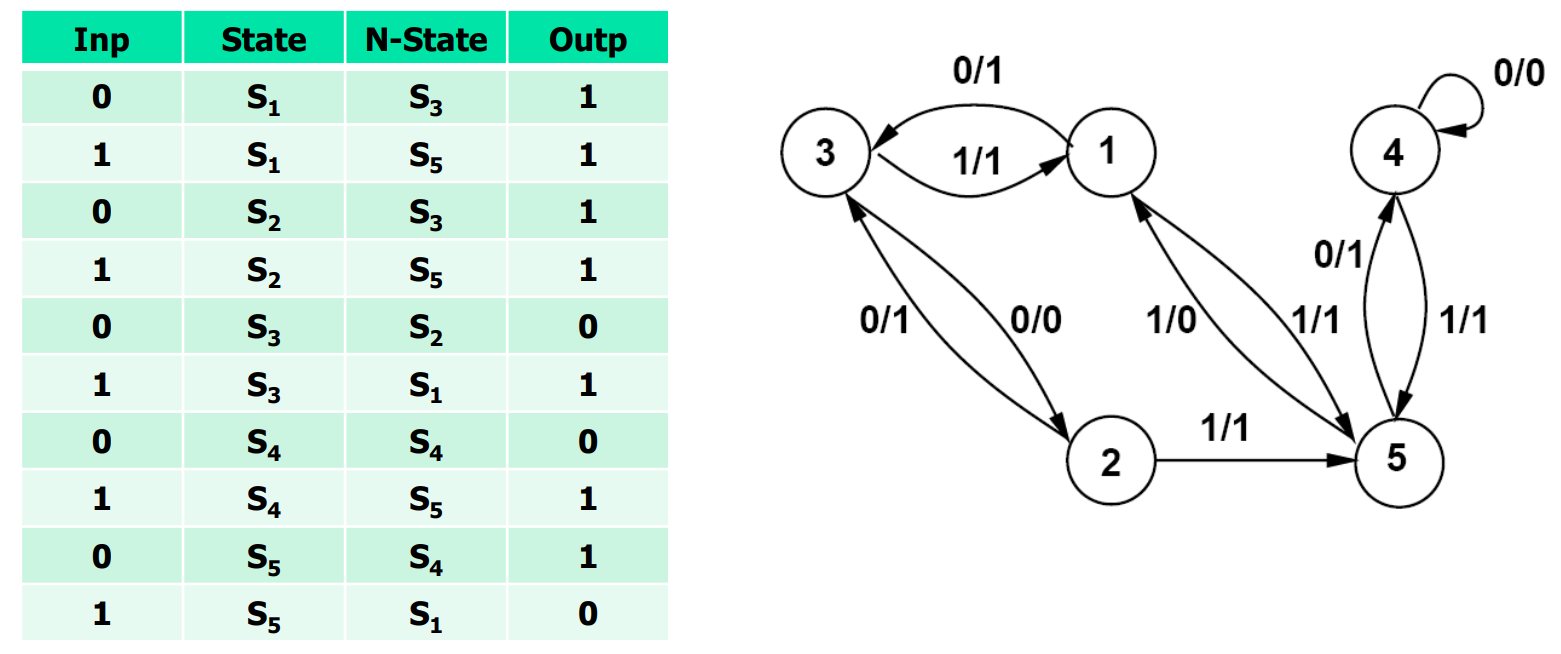
\includegraphics[width=11cm, scale=1]{S2/stateMinimization_CS.PNG}
    \caption{Perform state minimization on this completely-specified state model}
\end{figure}

\begin{enumerate}
    \item $\Pi_{0} = \left\{ S_{1},S_{2}, S_{3}, S_{4}, S_{5} \right\} $
    \item $\Pi_{1} = \left\{ S_{1},S_{2} \right\},  \left\{ S_{3},S_{4} \right\}, \left\{ S_{5} \right\}$; Partition based on Output
    \item $\Pi_{2} = \left\{ S_{1},S_{2} \right\},  \left\{ S_{3},S_{4} \right\}, \left\{ S_{5} \right\}$; Iterative partition 0, consider $S_{i} = S_{1}, S_{j} = S_{2}$
        \begin{itemize}
            \item Consider Input = 0 for $\left\{ S_{1},S_{2} \right\}$.
                \begin{itemize}
                    \item $S_{1}$'s next-state is $S_{3}$, $S_{2}$'s next-state is $S_{3}$
                    \item $S_{3}$ must be equivalent to $S_{3}$, since they are the same state
                \end{itemize}
            \item Consider Input = 1 for $\left\{ S_{1},S_{2} \right\}$.
                \begin{itemize}
                    \item $S_{1}$'s next-state is $S_{5}$, $S_{2}$'s next-state is $S_{5}$
                    \item $S_{5}$ must be equivalent to $S_{5}$, since they are the same state
                \end{itemize}
            \item Therefore, $S_{1}$ equivalent to $S_{2}$ (and grouped in the same 'block')
        \end{itemize}
    \item $\Pi_{3} = \left\{ S_{1},S_{2} \right\},  
                     \left\{ S_{3} \right\}, 
                     \left\{ S_{4} \right\}, 
                     \left\{ S_{5} \right\}$; Iterative partition 1, consider $S_{i} = S_{3}, S_{j} = S_{4}$
        \begin{itemize}
            \item Consider Input = 0 for $\left\{ S_{3},S_{4} \right\}$.
                \begin{itemize}
                    \item $S_{3}$'s next-state is $S_{2}$, $S_{4}$'s next-state is $S_{4}$
                    \item Is $S_{2}$ equivalent to $S_{4}$? No, since they were not in the same 'block' for $\Pi_{2}$
                \end{itemize}
            \item Therefore, $S_{3}$ cannot be equivalent to $S_{4}$ (and they must be grouped in seperate 'blocks')
        \end{itemize}
    \item No furthur refinement can be made to $\Pi_{3}$, therefore we have reached convergence and achieved state minimization.
\end{enumerate}

\newpage
\subsubsection{State Minimization - Incompletely specified FSMs}
Note: The resulting "minimized" FSM is \textbf{not unique}.

\paragraph{Concept of \textit{compatible} states}
\begin{itemize}
    \item Assume we have two states $S_{1}$ and $S_{2}$. $S_{1}$ and $S_{2}$ defined as \textit{compatible} iff for some \textbf{applicable} input sequence \dots
        \begin{itemize}
            \item Their (combinational) outputs are identical \textbf{if specified}, and
            \item Their (combinational) next-states are \textit{compatible} (note the recursiveness) as well
        \end{itemize}
    \item The key difference in this definition, is that the input sequence must be \textbf{applicable}, before we can even consider whether the outputs are identical (if they are even \textbf{specified} at all)
        \begin{itemize}
            \item An inapplicable input is one where it is don't-care (X). By definition, we then wouldn't care what it's output is.
            \item Only if the input is applicable, do we have to consider whether the output is identical/next-state is compatible 
            \item An example is shown in Fig7 below. FSM\_B receiving an 'X', means the particular input (outputted from FSM\_A) is guaranteed not to happen (that's why it's 'X' in the first place). So we need not bother with what FSM\_B outputs in this case.
        \end{itemize}
        \begin{figure}[htp]
            \centering
            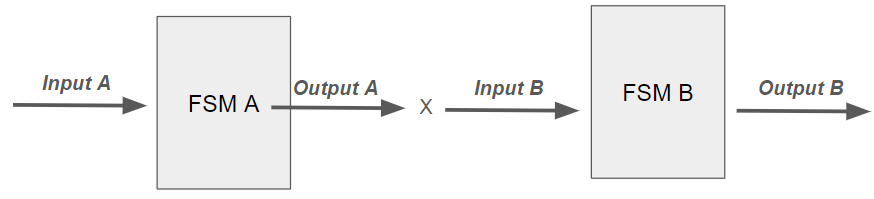
\includegraphics[width=6cm, scale=1]{S2/dontCareOutputInput.PNG}
            \caption{Propagation of 'X' from FSM\_A to FSM\_B}
        \end{figure}
    \item Note that compatibility is \textbf{not} transitive. We will prove this via example.
        \begin{itemize}
            \item Suppose for a particular input; $S_{1}$ has output 10, $S_{2}$ has output 1*, $S_{3}$ as output 11
                \begin{itemize}
                    \item $S_{1}$ compatible with $S_{2}$, assuming their next-states are compatible
                    \item $S_{2}$ compatible with $S_{3}$, assuming their next-states are compatible
                    \item $S_{1}$ not compatible with $S_{3}$, irregardless of their next-states. Thereby proving transitivity doesn't hold.
                \end{itemize}
        \end{itemize}
\end{itemize}

\paragraph{Algorithm for State Minimization of IS-FSMs}

\begin{enumerate}
    \item n don't cares implies $2^{n}$ CS-FSMs
    \item Hence, we have to iterate through and minimize $2^{n}$ possible CS-FSMs, to find the minimized IS-FSM
\end{enumerate}

\vspace{0.5cm}
Let's examine an example.

\begin{figure}[htp]
    \centering
    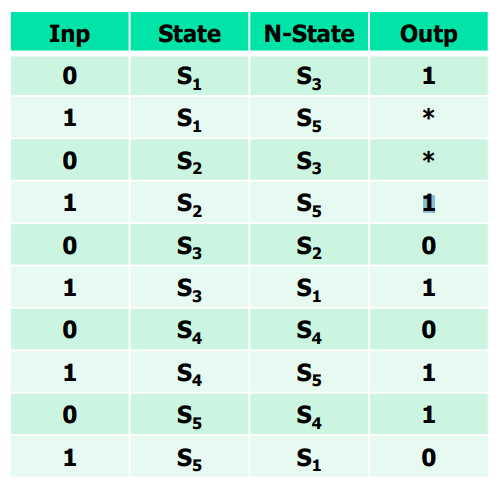
\includegraphics[width=6cm, scale=1]{S2/stateMinimization_IS.PNG}
    \caption{Perform state minimization on this incompletely-specified state-based model}
\end{figure}

\begin{itemize}
    \item One possible CS-FSM: Replace all '*' with '1'; (ie. The previous example on CS-FSM)
        \begin{itemize}
            \item $\Pi_{convergence} = \left\{ S_{1},S_{2} \right\},  
                                       \left\{ S_{3} \right\},
                                       \left\{ S_{4} \right\}, 
                                       \left\{ S_{5} \right\}$;
        \end{itemize}
    \item Another possible CS-FSM: Replace all '*' with '0'; 
        \begin{itemize}
            \item $\Pi_{convergence} = \left\{ S_{1},S_{5} \right\},
                                       \left\{ S_{2},S_{3},S_{4} \right\}$
            \item Intuitively, we can see that replacing all '*' with '0' results in a better minimization.
                  This is because there are less possible output combinations, therefore more terms are grouped 'in the same block' in $\Pi_{1}$.
        \end{itemize}
    \item Another possible CS-FSM: Replace $1^{st}$ '*' with '0', $2^{nd}$ '*' with '1'; 
        \begin{itemize}
            \item Intuitively, you can see that this will result in a worse minimization.
                  Using the same logic as before, this is because now there are more possible output combinations.
        \end{itemize}
\end{itemize}

\paragraph{Important difference between Equivalence and Compatible}\mbox{}\\\\
We already know that equivalence is transitive, compatible is non-transitive.
However, we also note that the following important difference
\begin{itemize}
    \item If $S_{1}$ and $S_{2}$ are 'truly' equivalent (ie. belonging to the same 'group' from $\Pi_{2}$ onwards), 
          then they \textbf{will} be grouped together in the final optimized minimized CS-FSM (ie. belonging to the same 'group' in $\Pi_{convergence}$)
    \item Even if $S_{1}$ and $S_{2}$ are 'truly' compatible (ie. belonging to the same 'group' from $\Pi_{2}$ onwards), 
          they \textbf{might not} be grouped together in the final optimized minimized IS-FSM (ie. might belong to different 'groups' in $\Pi_{convergence}$)
          \begin{itemize}
            \item You can observe this from the Fig8 example on IS-FSM.
            
                  $S_{1}$ and $S_{2}$ are 'truly' compatible, yet they do not belong to the 'best' minimized IS-FSM (corresponding to when we replace all '*' with '0')
          \end{itemize}
\end{itemize}

\paragraph{Compatibility and Implications}\mbox{}\\\\
Note: Implications also exist in the case of Equivalence, we are just explaining it wrt Compatibility context now.

There is a notion of 'implicit compatibility', where claiming $S_{i}$ and $S_{j}$ are compatible \textit{implies} that $S_{m}$ and $S_{n}$ are compatible.
Referring back to the Fig8 example \dots

\begin{itemize}
    \item $\left\{S_{3},S_{4}\right\}$ are compatible 
          $\xleftrightarrow{implies}$ 
          $\left\{S_{2},S_{4}\right\}$ are compatible
          $\wedge$
          $\left\{S_{1},S_{5}\right\}$ are compatible
\end{itemize}

\subsubsection{Formal definition of the State Minimization problem}
We want to find the minimal number of partition groups st \dots
\begin{enumerate}
    \item All states are covered (ie. Every state $S_{i}$ belongs to some group $\phi_{j}$ in our final partition $\Pi_{convergence}$)
    \item All implications are satisfied (we term this the \textit{closure} property)
\end{enumerate}

Exact solutions are computationally expensive, but good approximation methods do exist (not covered).

\subsection{State Encoding (Revisited)}
As seen in Section 2.2, State Encoding is the process of assigning bit-vectors to each symbolic state.

\subsubsection{How many possible ways are there to do State Encoding?}
Rewriting the question; Given \textit{m} states and \textit{n} bits, how many possible state-assignments are there?
\begin{itemize}
    \item We know that the \textit{minimal} number of bits required to encode \textit{m} states is \textit{n} = \textit{ceil}$\Bigl( log_{2}(m) \Bigr)$ bits
    \item Therefore with the lower limit in-place, we have \textit{n} $\ge$ \textit{ceil}$\Bigl( log_{2}(m) \Bigr)$
    \item Now let's work out how many ways there are to encode some state $S_{i}$, i $\le$ m
    \begin{enumerate}
        \item We have $2^{n}$ possible ways to encode the \textit{first} state $S_{1}$
        \item We have $2^{n}-1$ possible ways to encode the \textit{second} state $S_{2}$; One permutation is already taken up by $S_{1}$
        \item We have $2^{n}-2$ possible ways to encode the \textit{third} state $S_{3}$; Two permutations are already taken up by $S_{1},S_{2}$
        \item I think you get the pattern \dots
    \end{enumerate}
    \item Therefore, we have $\Bigl( (2^{n}) * (2^{n}-1) * (2^{n}-2) * \dots * (2^{n}-(m+1)) \Bigr) = \frac{(2^{n})!}{(2^{n}-m)!}$ possible ways to encode \textit{m} states using \textit{n} bits
\end{itemize}

\newpage
\subsubsection{Optimal state encoding}
With such a large solution space, which is the \textit{optimal} one? Well, it depends on what you are trying to optimize for.

\begin{itemize}
    \item 
    For example, if we are trying to optimize for size (amount of combinational logic and number of FFs),
    we might choose \textit{n} = \textit{ceil}$\Bigl( log_{2}(m) \Bigr)$; i.e Lowest number of FFs required to encode all states. 
        \begin{itemize}
            \item Subsequently we could perform \textit{sequential} encoding, where we encode states in an incremental binary fashion. \newline
                  eg. $S_{1} \xrightarrow{} 000$ , $S_{2} \xrightarrow{} 001$, $S_{3} \xrightarrow{} 010$, $S_{4} \xrightarrow{} 011$
        \end{itemize}
    \item
    However, we might also choose to optimize for speed (Depth of combinational logic and fanout), in which-case the lowest number of FFs might not be ideal.
    One popular method to optimize for speed is utilizing \textit{One-Hot Encoding}.
\end{itemize}

\paragraph{One-Hot Encoding}\mbox{}\\\\
One-Hot Encoding utilizes as many FFs as there are states, and assigns in a one-hot manner. \newline
eg. $S_{1} \xrightarrow{} 0001$ , $S_{2} \xrightarrow{} 0010$, $S_{3} \xrightarrow{} 0100$, $S_{4} \xrightarrow{} 1000$

The main advantage of One-Hot Encoding, is that it reduces (might not optimally reduce, but still reduces) the complexity/area of the resulting combinational logic. Let's why.

\begin{itemize}
    \item Suppose we have 6 states $\left\{S_{1},S_{2},\dots,S_{6}\right\}$ in an FSM.
    \item Implementing in sequential encoding method, we use 3 FFs $\left\{FF_{1},FF_{2},FF_{3}\right\}$, resulting in the circuit below.
        \begin{figure}[htp]%
            \centering
            \subfloat[\centering Sequential Encoding to determine state $S_{1}$]{{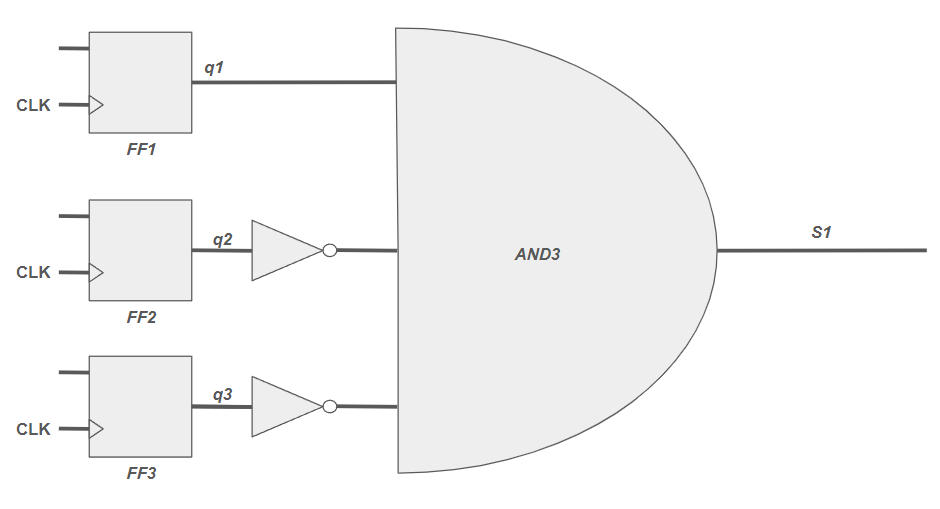
\includegraphics[width=9cm]{S2/sequentialEncoding.PNG}}}% 
            \qquad
            \subfloat[\centering 3AND is formed from 2 2AND]{{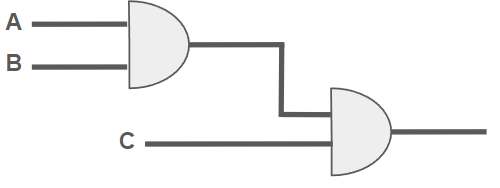
\includegraphics[width=9cm]{S2/threeAnd.PNG}}}% 
            \caption{Sequential Encoding saves on FFs, but has more combinational delay}%
        \end{figure}
    \item Implementing in one-hot encoding method, we use 6 FFs $\left\{FF_{1},FF_{2}, \dots, FF_{6}\right\}$, resulting in the circuit below.
        \begin{figure}[htp]
            \centering
            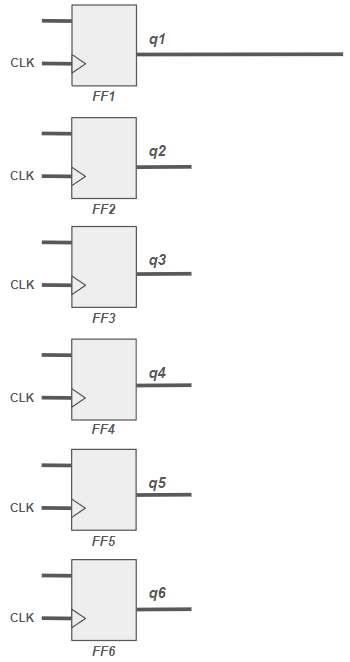
\includegraphics[width=5cm, scale=1]{S2/oneHotEncoding.PNG}
            \caption{One-Hot Encoding to determine state $S_{2}$; Splurges on FFs, but less combinational delay}
        \end{figure}
\end{itemize}

\subsubsection{Heuristics for State Minimization}
The problem of \textit{optimal} state minimization is intractable as mentioned previously.
Therefore, we need to rely on heuristic methods for practical applications.

Most of these heuristic methods rely on assiging \textbf{adjacent codes} to states that are very 'similar',
with adjacent codes having the property of requiring only one bit change for each successive state in a counting sequence.

The purpose of using adjacent codes is because simplification using K-Maps will be better.
\begin{itemize}
    \item Adjacent codes (1bit difference in the binary assignment) causes 1s to be placed beside each other in the K-Map
    \item A bigger 'cluster' of 1s in the K-Map means that more variables can be grouped together, and more simplification can be done
\end{itemize}

\begin{figure}[htp]%
    \centering
    \subfloat[\centering Truth table for some FSM]{{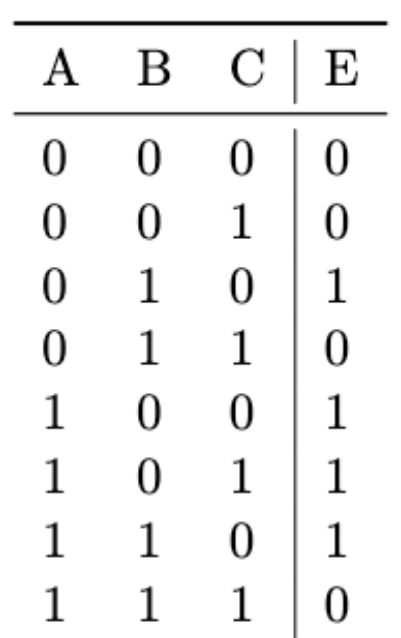
\includegraphics[width=4cm]{S2/adjacentCodeTruthTable.PNG}}}% 
    \qquad
    \subfloat[\centering K-Map, notice that the adjacent codes in the FSM are located side-by-side and allowing for greater 'clustering']{{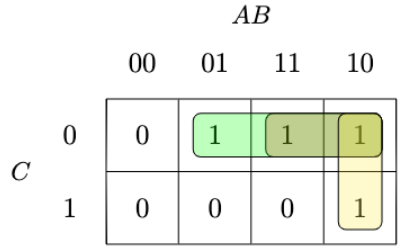
\includegraphics[width=9cm]{S2/adjacentCodeKMap.PNG}}}% 
    \caption{Showing why adjacent codes result in better K-Map simplification}%
\end{figure}


Some examples would be \dots
\begin{itemize}
    \item Clustering of 1s in next-state K-Map
        \begin{itemize}
            \item Assigning adjacent codes to states that share a \textit{common next-state}
            \item Assigning adjacent codes to states that share a \textit{common predecessor-state}
        \end{itemize}
    \item Clustering of 1s in output K-Map
        \begin{itemize}
            \item Assigning adjacent codes to states that have a \textit{common output behavior}
        \end{itemize}
\end{itemize}


Popular choices for adjacent codes are \textit{Gray Codes} and \textit{Johnson Codes}.

\subsection{State Extraction}
Not covered in detail, but the basic idea is straight-forward.

\begin{itemize}
    \item A circuit with \textit{n} FFs has $2^{n}$ states, however not all states may be reachable
        \begin{itemize}
            \item eg. Suppose we have 3 FFs implementing 3 states, in a one-hot encoding scheme
                \begin{itemize}
                    \item Legal states are only 001,010,100
                \end{itemize}
        \end{itemize}
    \item Therefore, there is a need to verify whether our structural model erroneously enters an illegal state
\end{itemize}

\subsubsection{State Extraction Algorithm}
\begin{enumerate}
    \item Find all states reachable from the initial state, and add these states to the set of reachable states
        \begin{itemize}
            \item Note that we are able to find next-state from current-state, since we have the combinational expression for next-state generation from our structural model
        \end{itemize}
    \item From this set, determine all it's reachable states, and add these states to the set of reachable states
    \item Repeat above step until convergence is reached (no new reachable states can be added to set)
\end{enumerate}

\newpage
\subsection{Retiming}
EE4415 covers this in much greater detail.

\subsubsection{Synchronous Network Graph (SNG)}
\begin{itemize}
    \item Vertices: SOP/POS combinational logic; \textit{Logic gates}
    \item Edge weight: Synchronous delay; \textit{Registers/FFs}
    \item Edge direction: Dependencies; \textit{Nets}
\end{itemize}

\begin{figure}[htp]
    \centering
    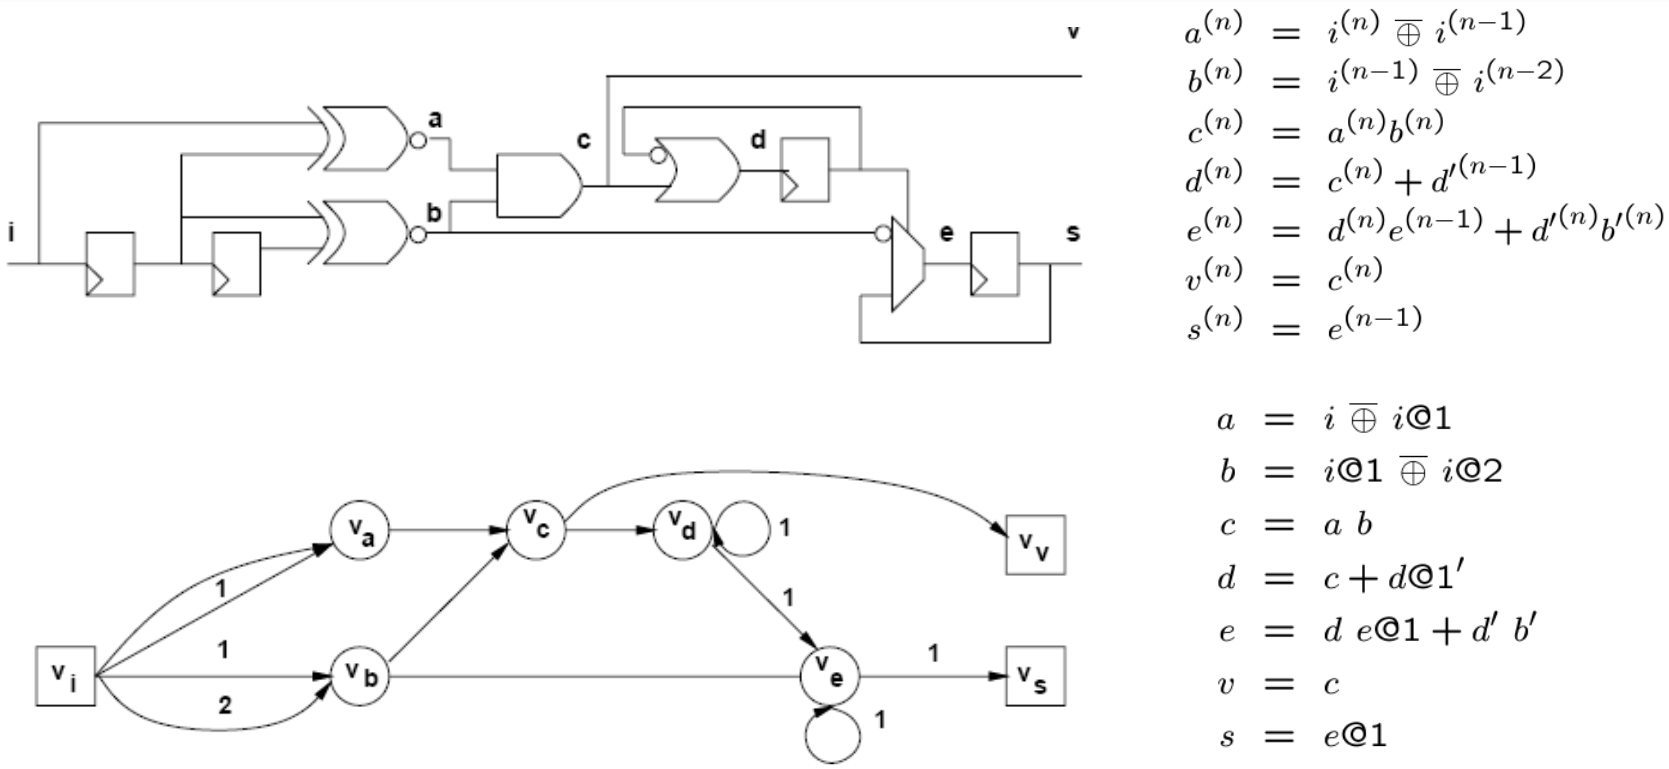
\includegraphics[width=19cm, scale=1]{S2/syncNetworkGraph.PNG}
    \caption{SNG derived from a structural model}
\end{figure}

\subsubsection{Basic concept of Retiming}
Rearranging of register positions to either reduce \textit{critical path delay} \textbf{OR} \textit{register count} is termed Retiming.

\begin{figure}[htp]%
    \centering
    \subfloat[\centering Reduced register count]{{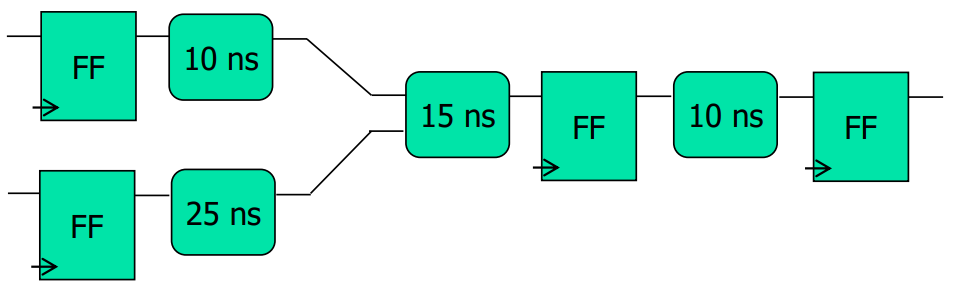
\includegraphics[width=9cm]{S2/recall_retiming0.PNG}}}% 
    \qquad
    \subfloat[\centering Reduced critical path delay]{{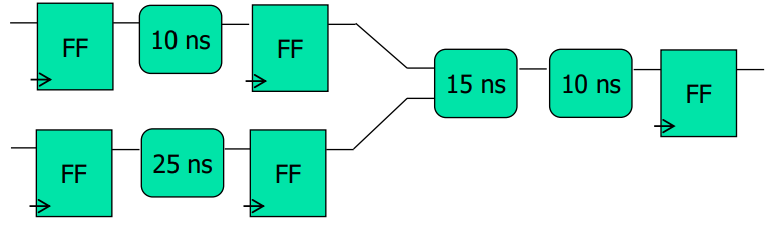
\includegraphics[width=9cm]{S2/recall_retiming1.PNG}}}% 
    \caption{Register Retiming for different optimization targets}%
\end{figure}

Note that retiming still maintains the original \textbf{system} functionality (ie. Delay between I/O does not change).

Observe the example in Fig14, where we do \textit{backward} retiming.

\newpage
\subsubsection{Retiming on the SNG}
Retiming is best understood from the SNG's POV.
\begin{figure}[htp]%
    \centering
    \subfloat[\centering Original]{{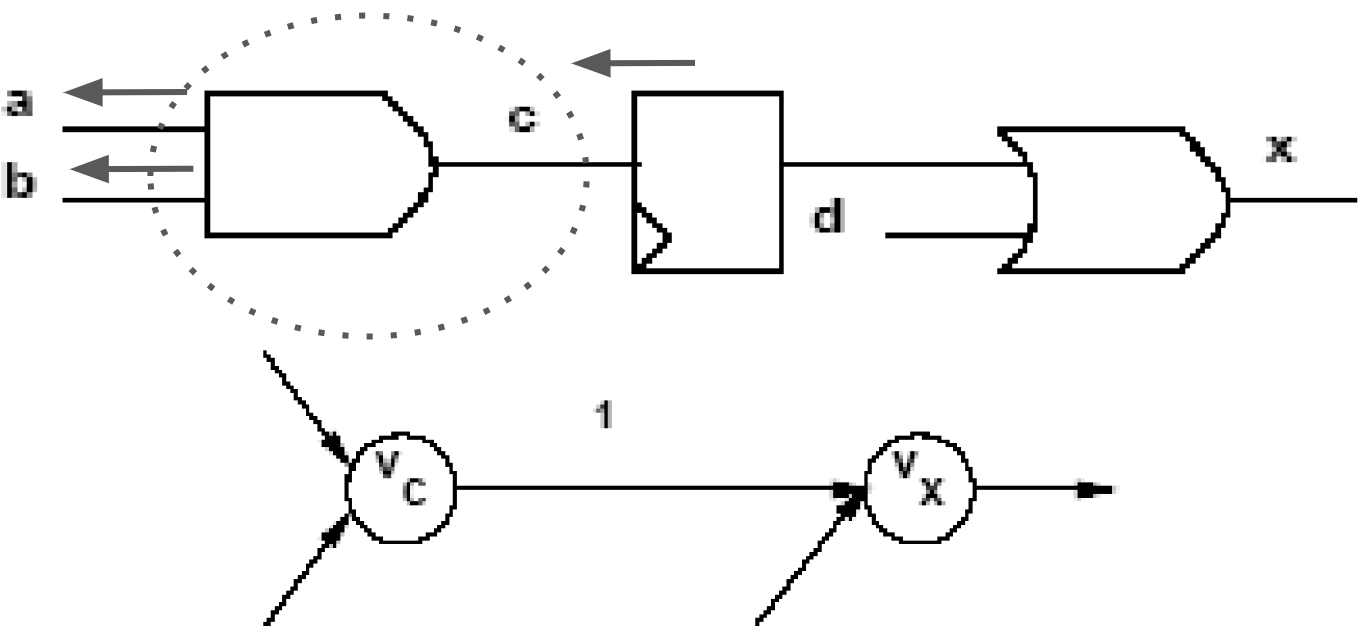
\includegraphics[width=9cm]{S2/SNG_retiming0.PNG}}}% 
    \qquad
    \subfloat[\centering Backward-retimed]{{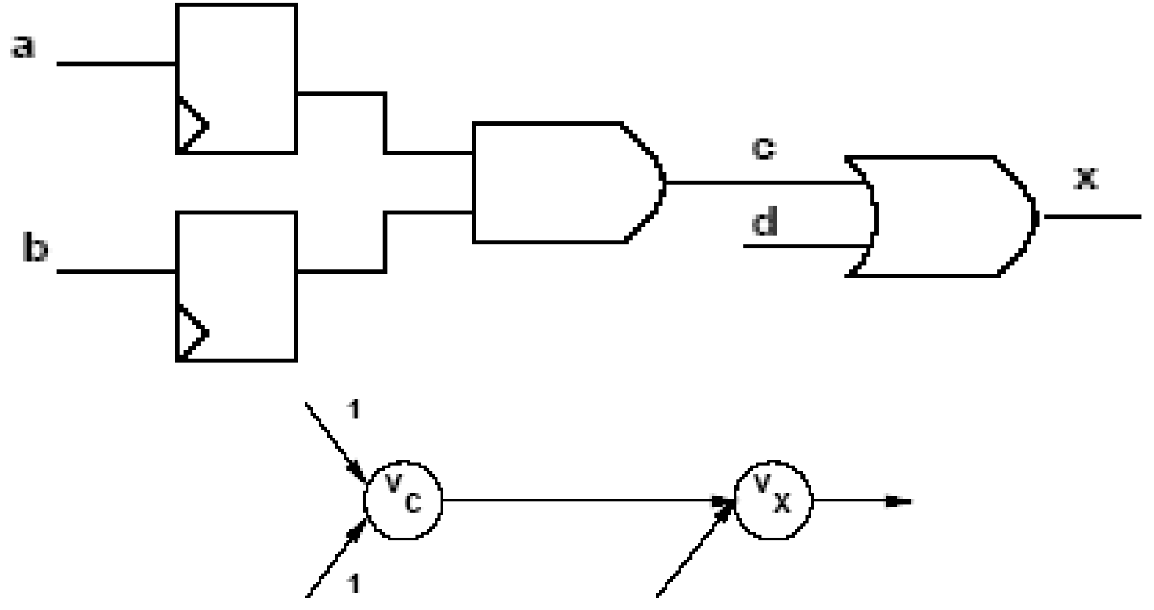
\includegraphics[width=9cm]{S2/SNG_retiming1.PNG}}}% 
    \caption{Backward Retiming (remove register from output, insert registers at input)}%
\end{figure}

For all cases of retiming (\textit{forward} or \textit{backward}) retiming, we observe that \dots
\begin{itemize}
    \item Network topology is preserved
    \item Area is affected (register count is changed)
    \item Clock frequency is affected (path delays between register pairs are changed)
        \begin{itemize}
            \item If \textit{critical} path delay is reduced, then clock frequency is increased as a result
            \item We note that path delays between I/O register pairs \textbf{must not} be changed, to preserve system functionality
        \end{itemize}
\end{itemize}

\paragraph{Retiming assumptions}
\begin{enumerate}
    \item \textbf{Cycles} must have positive weights (ie. No combinational feedback loop can exist)
        \begin{itemize}
            \item This is because register retiming on a recursive DFG (ie. one with a loop) \textbf{alters} the system functionality, which is unacceptable
            \item Therefore, any combinational feedback loop must be broken by at least one register.
        \end{itemize}
        \begin{figure}[htp]%
            \centering
            \subfloat[\centering Combinational feedback loop]{{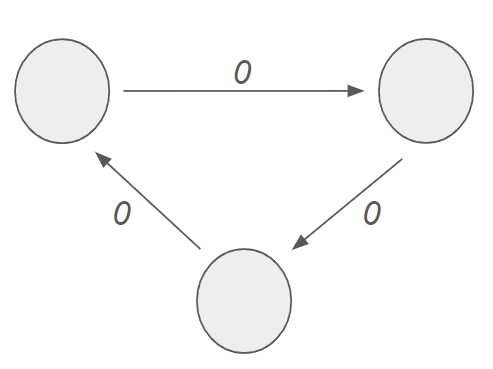
\includegraphics[width=4cm]{S2/combFeedLoop.PNG}}}% 
            \qquad
            \subfloat[\centering Broken combinational feedback loop]{{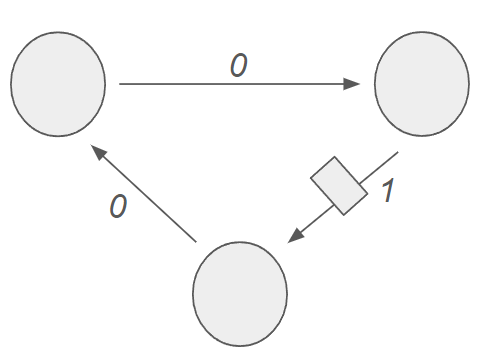
\includegraphics[width=4cm]{S2/combFeedLoop_Broken.PNG}}}% 
            \caption{Breaking of combinational feedback loop using registers}%
        \end{figure}
    \item Edges must have non-negative weights
    \item Combinational logic (ie. vertices) have no fan-out delay dependency (ie. Delay is independent of loading)
        \begin{figure}[htp]%
            \centering
            \subfloat[\centering Input vertex has fanout of 2]{{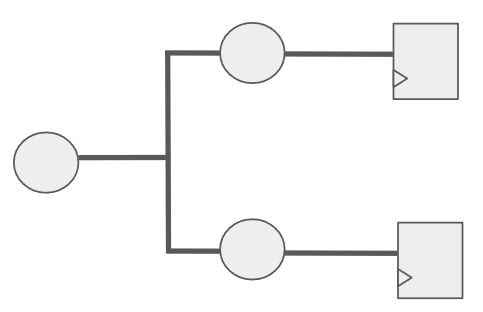
\includegraphics[width=5cm]{S2/fanout1.PNG}}}% 
            \qquad
            \subfloat[\centering Input vertex has fanout of 1 ]{{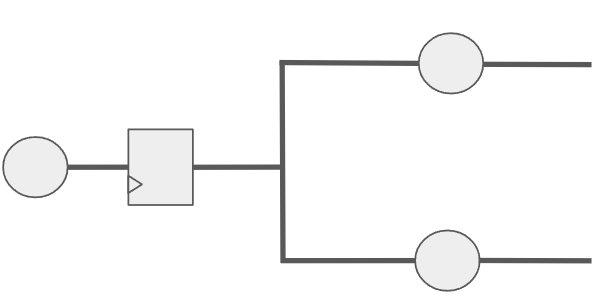
\includegraphics[width=5cm]{S2/fanout2.PNG}}}% 
            \caption{Vertex fan-out}%
        \end{figure}
    \item No false path analysis
\end{enumerate}

\paragraph{Retiming on SNG}\mbox{}\\\\
Note: Critical path is always calculated from some \textit{launching} register to a \textit{capturing} register
    \begin{figure}[htp]%
        \centering
        \subfloat[\centering Original; Critical delay=24]{{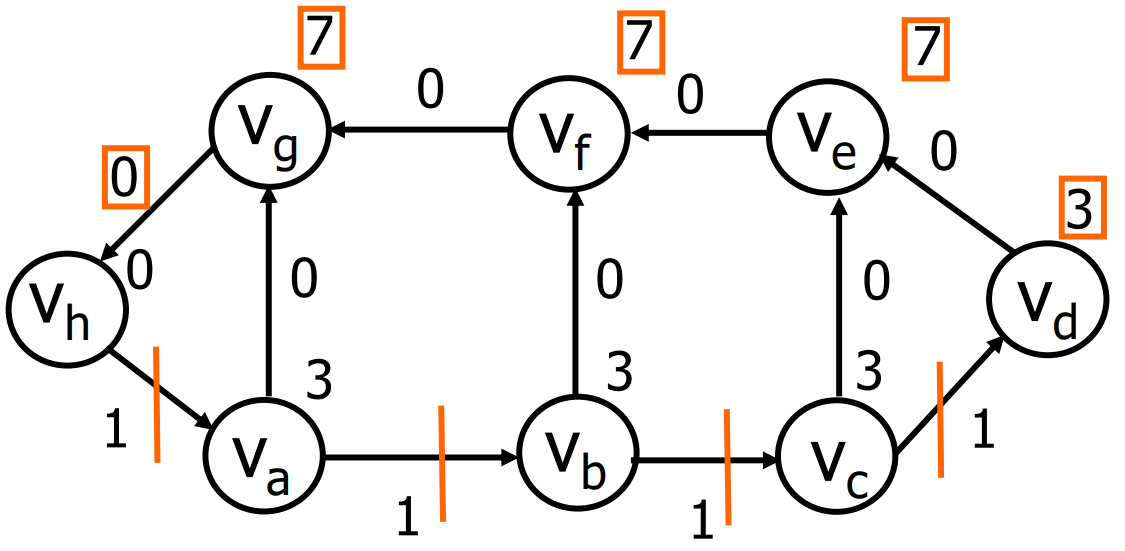
\includegraphics[width=8cm]{S2/retiming_eg1_1.PNG}}}% 
        \qquad
        \subfloat[\centering Retimed; Critical delay=13]{{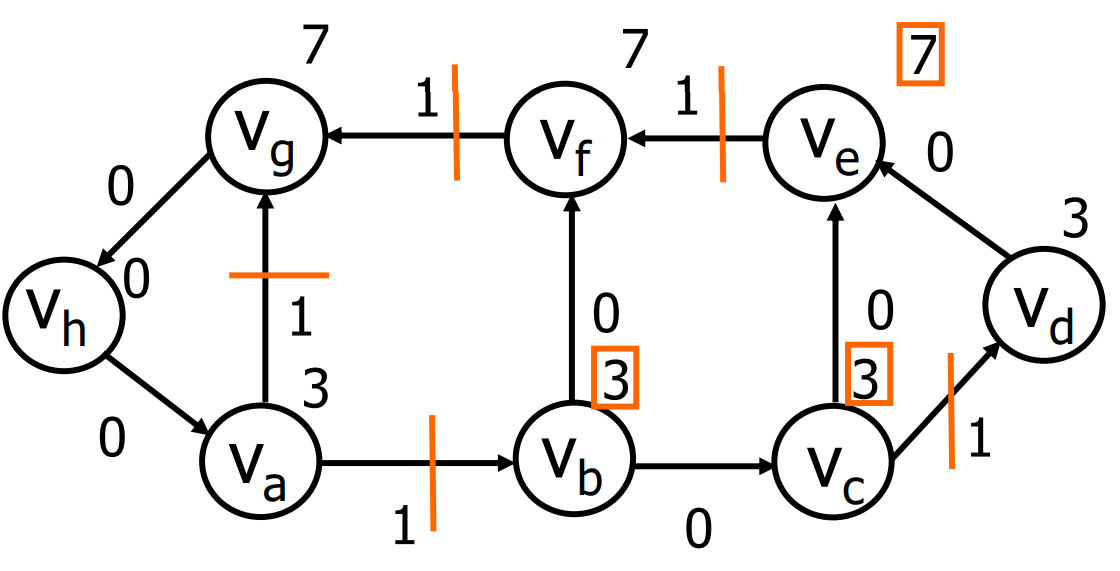
\includegraphics[width=8cm]{S2/retiming_eg1_2.PNG}}}% 
        \caption{Retiming on SNG}%
    \end{figure}

Furthur note that for the same critical delay, the corresponding retimed graph is \textbf{not} unique.


\paragraph{Relaxation-based retiming}\mbox{}\\\\
Idea is to look for paths with excessive delays, and reduce the delay via retiming (ie. Insert registers along the path)

\begin{enumerate}
    \item Start with a desired cycle-time $\varphi$ that we wish to achieve
    \item Find vertices $\left\{ v_{1}, v_{2}, \dots, v_{j} \right\}$ with \textit{data ready} $> \varphi$
        \begin{itemize}
            \item \textit{data ready} of a vertex $v_{i}$ is defined as
                  $\Bigl( (\text{delay from a } \textbf{register } \text{to } v_{i}) + (\text{weight of vertex } v_{i}) \Bigr)$
        \end{itemize}
    \item Iteratively retime these vertices $\left\{ v_{1}, v_{2}, \dots, v_{j} \right\}$
        \begin{itemize}
            \item Since register retiming must 'take' registers from somewhere, other paths may become longer
            \item Also ensure that no edge has negative weight after 'taking' of registers
        \end{itemize}
    \item If at some iteration $\Phi_{k}$ there is no vertex $v_{i}$ with \textit{data ready} $> \varphi$, then a legal retiming has been found
        \begin{itemize}
            \item We might further optimize by choosing a smaller $\varphi$, and repeating the process
        \end{itemize}
    \item If a legal retiming is not found by iteration $\Phi_{m}$ where \textit{m} is our chosen \textit{iteration bound}, then no legal retiming exists for that $\varphi$
        \begin{itemize}
            \item Try again with a larger $\varphi$ 
        \end{itemize}
\end{enumerate}


\paragraph{Relaxation retiming on SNG}\mbox{}\\
Assume that our goal is to have $\varphi = 13$
\begin{enumerate}
    \item Remove all edges with weight $\ge$ 1, to identify \textit{data ready} of vertices better
    \item We identify that $v_{f}$ has a \textit{data ready} of 17, let's retime that first
    \begin{figure}[htp]
        \centering
        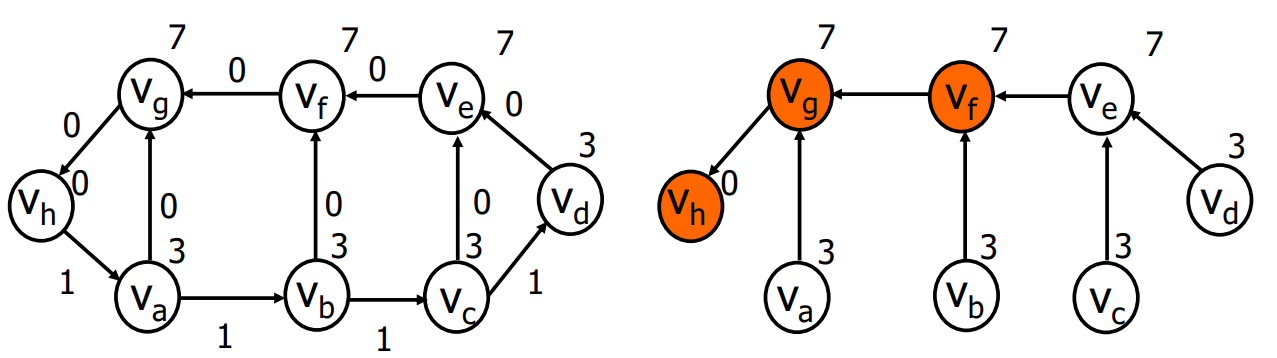
\includegraphics[width=14cm, scale=1]{S2/relaxationRetime1.PNG}
        \caption{Iteration $\Phi_{1}$}
    \end{figure}
    \newpage
    \item We have retimed $v_{f}$ accordingly. Now simply repeat the previous steps to identify that $v_{g}$ needs to be retimed now.
    \begin{figure}[htp]
        \centering
        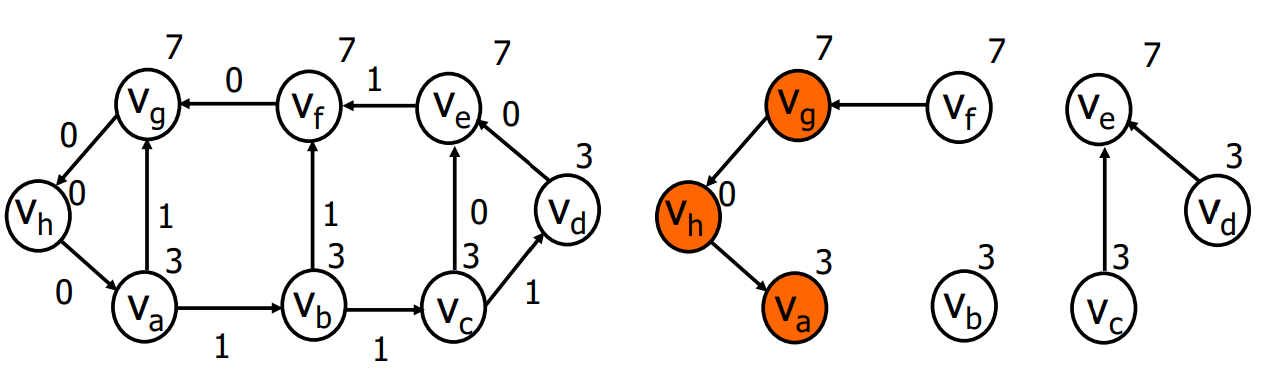
\includegraphics[width=14cm, scale=1]{S2/relaxationRetime2.PNG}
        \caption{Iteration $\Phi_{2}$}
    \end{figure}
    \item We have retimed $v_{g}$ accordingly, and reached our desired $\varphi$
    \begin{figure}[htp]
        \centering
        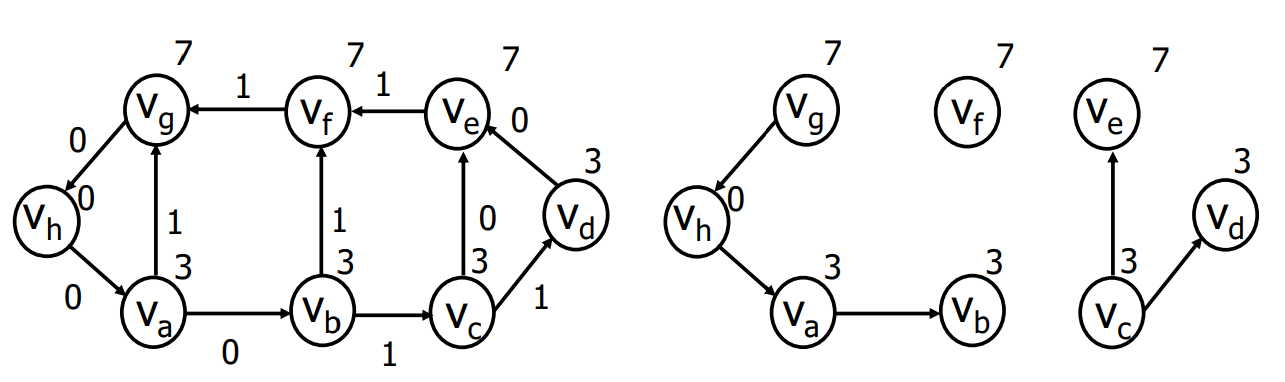
\includegraphics[width=14cm, scale=1]{S2/relaxationRetime3.PNG}
        \caption{Iteration $\Phi_{3}$; Convergence}
    \end{figure}
\end{enumerate}

\paragraph{Retiming for minimal area}\mbox{}\\
Previously, all our discussion was on retiming for minimal \textit{delay}. We can also retime for minimal \textit{area}.

\begin{figure}[htp]
    \centering
    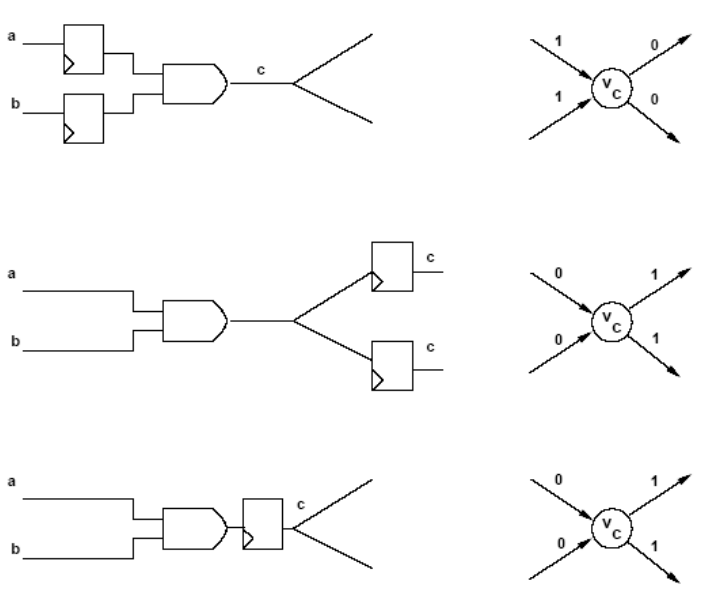
\includegraphics[width=10.5cm, scale=1]{S2/retime_minArea.PNG}
    \caption{Retiming for minimal area}
\end{figure}

\end{document}